%%%%%%%%%%%%%%%%%%%%%%%%%%%%%%%%%%%%%%%%%%%%%%%%%%%%%%%%%%%%%%%%%%%%%%%%
%                                                                      %
%     File: Thesis_StateOfTheArt.tex                                   %
%     Tex Master: Thesis.tex                                           %
%                                                                      %
%     Author: Gonçalo Santos                                           %
%     Last modified : 20 Oct 2018                                      %
%                                                                      %
%%%%%%%%%%%%%%%%%%%%%%%%%%%%%%%%%%%%%%%%%%%%%%%%%%%%%%%%%%%%%%%%%%%%%%%%

\chapter{State of the Art} % 20
\label{chapter:estadodaarte}

In this chapter a description of the current state of compiler frameworks and
their application to reconfigurable processors is presented. The chapter begins
by explaining the concept of Coarse Grained Reconfigurable Array ({\sc CGRA}), in
order to introduce the Versat reconfigurable processor. Then, several compiler
frameworks are studied with the purpose of selecting a tool for the development
of the Versat compiler. A section about {\sc CGRA} compilers and a comparative
analysis closes the chapter.


\section{CGRA}

A {\sc CGRA} is a programmable hardware structure made of coarse grained
components such as Arithmetic and Logic Units ({\sc ALUs}) whose function (add,
multiply, shift, {\it etc.}) and
interconnection can be programmed differently for
executing different applications~\cite{Tripp07}. {\sc CGRA}s can be controlled by one
or more host processors. By selecting the appropriate components the performance
can optimized, and the total power consumption can be significantly reduced.  The
wiring between the components can then be programmed prior to data
processing~\cite{Cao17TVLSI,Dave18DAC,Gu18TPDS}.  Recent developments allow the
configuration of address generators that implement nested loops in a few
instructions, reducing the configuration time of {\sc CGRA}s~\cite{deSutter10}.
Instead of using a single static configuration for each program, {\sc CGRA}s can
now be reconfigured multiple times during program execution, {\it i.e.} dynamic
reconfiguration~\cite{Hartenstein01}.  However, since reconfiguration consumes
execution time, a balance must be met in order to achieve good
performance~\cite{Mukherjee17VLSID}.

\section{Versat}
\label{section:versat}

{\it Versat} is a {\sc CGRA} architecture where each piece of the program being
executed can use a different composition of functional units~\cite{deSousa12}.
It is used as a hardware accelerator for embedded systems.  It uses a controller
to generate and update the configuration, the {\it picoVersat}.  The controller
is programmable and executes programs written in {\bf C} and assembly (specific
to the architecture).  Contrary to most {\sc CGRA}s, which can only be fully
reconfigured, {\it Versat} allows for partial reconfiguration (where only few
configuration bits are changed), thus optimizing configuration changes.
Moreover, in this approach the configurations are self-generated. Consequently,
the host does not have to manage the reconfiguration process and is free to
perform more useful tasks~\cite{Lopes2017}.  {\it Versat} uses an address
generation scheme that is able to support nested loops expressed in a single
{\sc CGRA} configuration.  Due to the better silicon area utilization and power
efficiency of heterogeneous {\sc CGRA}s architectures, when comparing to
homogeneous ones, an heterogeneous structure was adopted for {\it Versat}.

\subsection{Architecture}

{\it Versat} can be used by host processors in the same chip (allows for
procedures to run faster and with less power consumption), and was designed for
fixed-point signal processing. Its architecture itself is composed of five
different components and is shown in figure~\ref{fig:versat_arch}. These
components are a Controller, a Control Register File ({\sc CRF}), the Data
Engine ({\sc DE}), the Configuration Module ({\sc CM}), and the {\sc DMA}.


\begin{figure}[!htbp]
    \centerline{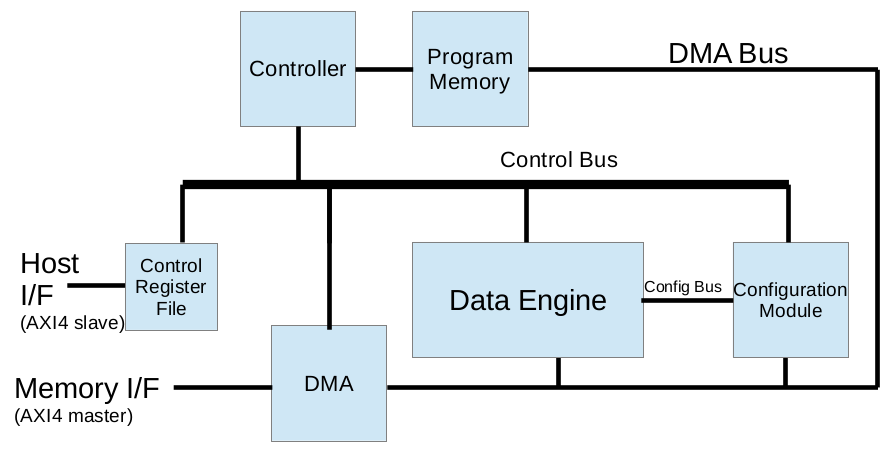
\includegraphics[width=0.8\textwidth]{Figures/top.png}}
    \vspace{0cm}\caption{{\it Versat} top-level architecture.}
    \label{fig:versat_arch}
\end{figure}

The Controller is a programmable component of the architecture that has a direct
dependency with the host that is controlling it, and is in charge of the data
flow, algorithm calculation, and control of the self configuration. The control
data is passed to the other sectors of {\it Versat} through a Control Bus like
for example the attached Serial Divider. The Controller that is used is called
{\it picoVersat}.  The {\sc DE} is the module that does the computations and is
composed of interconnected Functional Units ({\sc FUs}).  The {\sc CM} has the
configurations of the datapaths that are meant to be executed by the {\sc
  DE}. It also allows for partial reconfiguration and for the change of
configuration in runtime.  The {\sc DMA} is a module that works in parallel with
{\it Versat} and has the function of transferring the configurations, programs
and data needed for the execution to and from {\it Versat}.

\subsubsection{Data Engine ({\sc DE})}

The {\sc DE} has a fixed topology comprised of 15 Functional Units ({\sc FUs})
organized in a mesh as shown in figure~\ref{fig:data_engine}.

\begin{figure}[!htbp]
    \centerline{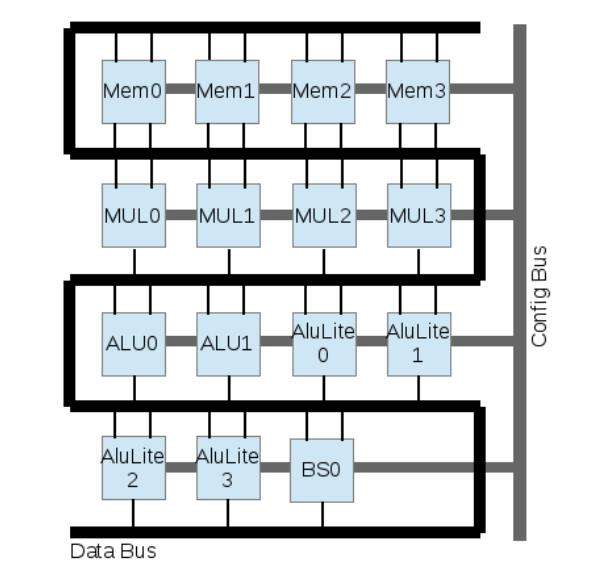
\includegraphics[width=0.7\textwidth]{Figures/DataEngine.jpg}}
    \vspace{0cm}\caption{Data Engine Structure.}
    \label{fig:data_engine}
\end{figure}

The {\sc DE} is a 32-bit architecture containing 15 {\sc FUs} which consist of
one barrel shifter, six {\sc ALUs}, four multipliers and four dual-port 8kB
embedded memories.  The system's Controller reads and writes from the {\sc FUs}
and to the memories.

Each {\sc FU} reads it's configuration of an operation and an input selection
from the Configuration Bus.  All {\sc FUs} write their 32 bit output to a wide
Data Bus of 19x32 bits.  The operations are chosen from a fixed number of those
that are available to the accelerator.

The {\sc DE} can be configured using one or more hardware datapaths, which
allows for Data Level Parallelism ({\sc DLP}) or Instruction level Parallelism
({\sc ILP}) depending on if the execution happens in parallel lanes or if the
paths are pipelined, respectively. Datapaths can operate in parallel in this
architecture as long as the resources needed to execute each of the datapaths are
available, which also gives {\it Versat} the capability of having Thread Level
Parallelism ({\sc TLP}).

Some of the most used cases of parallelism can be described by the following
examples of hardware datapaths.  In figure~\ref{fig:de_datapaths} there are
shown three examples of datapaths describing these cases of parallelism.

\begin{figure}[!htbp]
    \centerline{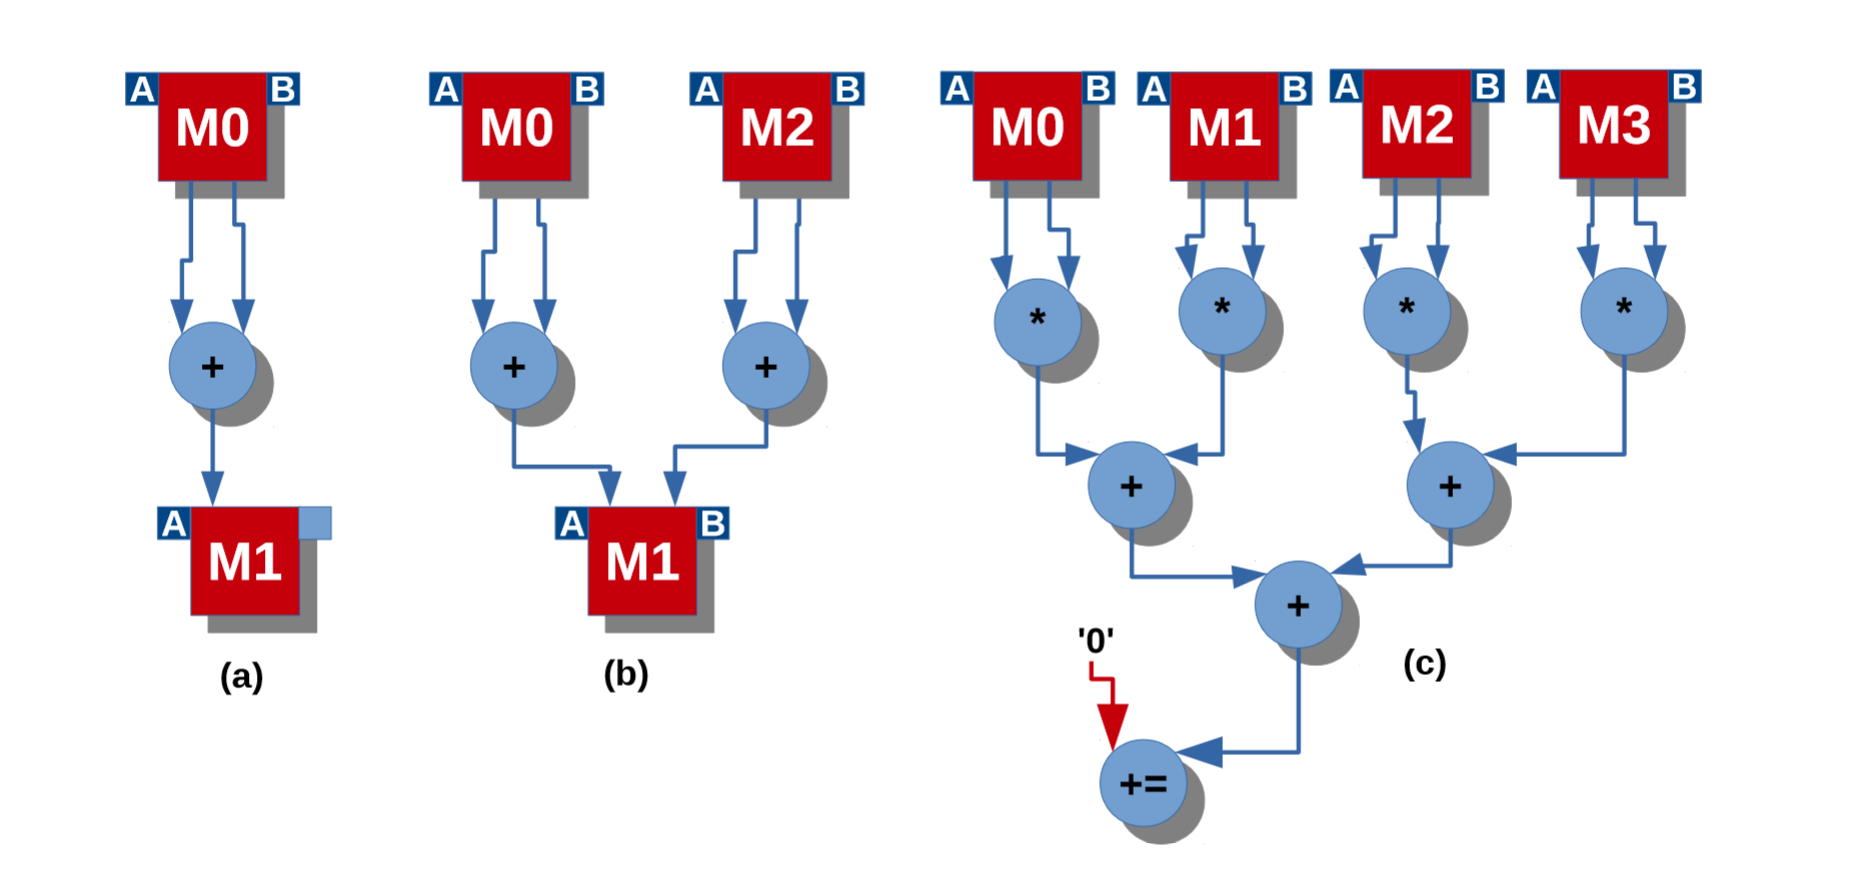
\includegraphics[width=0.8\textwidth]{Figures/de_datapaths.png}}
		\vspace{0cm}\caption{Data Engine Structure configuration examples with dual-port
		(A and B), memories (M0 to M3), and functional units (adders and multipliers).}
    \label{fig:de_datapaths}
\end{figure}

Because of the nature of the architecture, pipelined vector addition, the memory
read and write operation, and the addition operation, can be done in parallel, for
consecutive elements of that vector, as shown in (a).  It is possible to do
multiple pipelined vector addition operation using data from different memories
and saving the results in the same or different memories in parallel, if the
data itself is not dependent on each other, like in the case of (b).  When there
is a need to do the inner product of two vectors, since in this case elements
from each vector are multiplied, then the results are added and accumulated,
which is shown in datapath (c).  All of the {\sc ALU} operations described can
be executed in parallel~\cite{Lopes2017}.

There is an independent Address Generation Unit ({\sc AGU}) for each port of the
memories used, which allow for two level nested loops, and execution start with
a programmable delay.  {\sc TLP} can be exploited because the {\sc AGUs} can
operate independently, making it possible, for example, to operate through data
in different memories using two threads and then save the values obtained in the
same goal memory.
% explicar mais AGUs se for necessario

\subsubsection{Configuration Module}

The Configuration Module ({\sc CM}) is composed of three elements which are the
Configuration Register File ({\sc CRF}), the Configuration Shadow Register ({\sc
  CSR}) and the Configuration Memory ({\sc CM}), as shown in
figure~\ref{fig:config_module}.

\begin{figure}[!htbp]
    \centerline{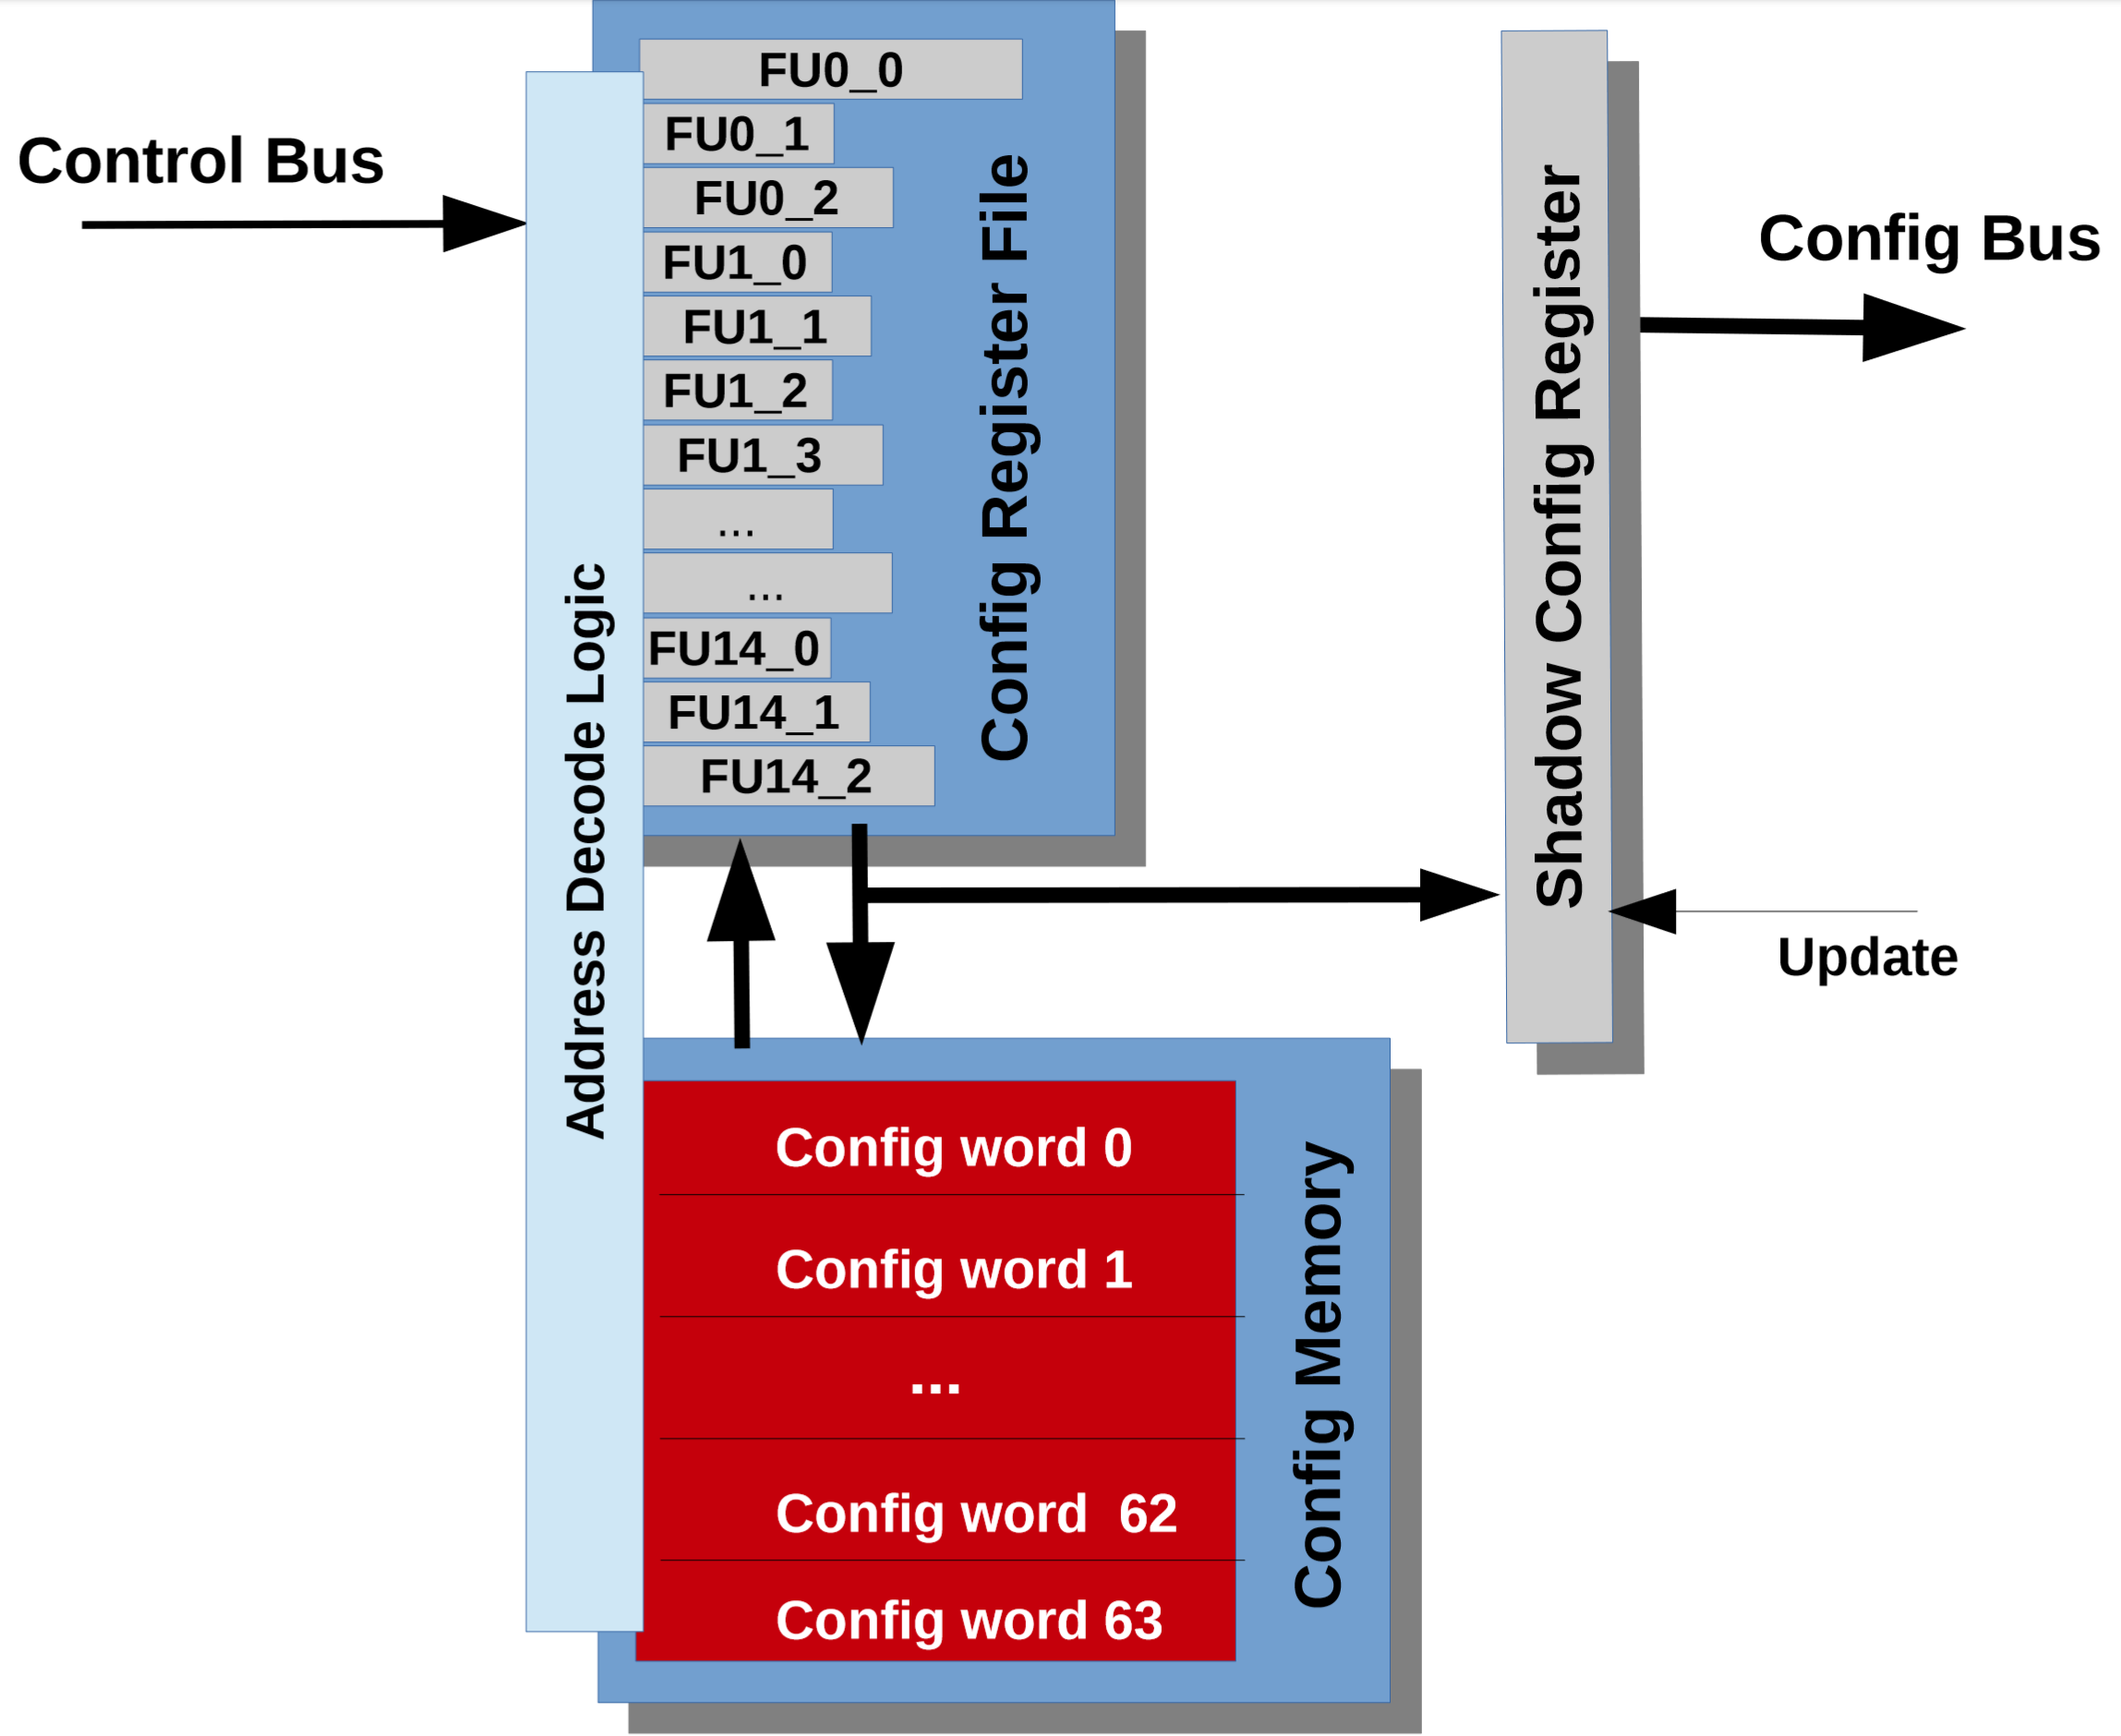
\includegraphics[width=0.7\textwidth]{Figures/config_module.png}}
    \vspace{0cm}\caption{Configuration Module Structure.}
    \label{fig:config_module}
\end{figure}

The preparation of the next configuration to be executed by the {\sc DE} is done
by the {\sc CRF}. It is an element composed of 118 configuration fields, and each
of these differ on the number of bits they define, totaling a full configuration
of 672 bits. By having each of these fields separate, it is possible to take
advantage of the fact that, during the execution of most of the application
code, there is a high chance that the {\sc DE} configurations used are very
similar to each other.  A partial reconfiguration can be done more effectively
since they differ in a low number of fields.

During execution, the current {\sc DE} configuration is present in the {\sc
  CSR}. This configuration is updated by copying the configuration in the {\sc
  CRF} to the {\sc CRS} when an {\it Update Signal} is sent by the
Controller. This allows for the reconfiguration of the system using the {\sc
  CRF} while the configuration in the {\sc CSR} is running (hidden
reconfiguration in runtime).

Because some {\sc DE} configurations are very common there is a dedicated memory
for the most common configurations. Each configuration has 672 bits this
in a dual-port 64 position memory. The configurations saved in this memory can
be loaded/stored from/to the {\sc CRF} in a single clock cycle through one of
the memory ports while the other port is 32-bits wide and is used to load/store
in an external memory by using the {\sc DMA}, so that the {\sc CM} is able to
exceed 64 positions.

\subsubsection{Controller} % 5
\label{section:picoversat}

{\it picoVersat} is a minimal hardware controller with a reduced instruction set
and few registers, with the purpose of doing simple calculations and giving
instructions to its connected systems. Therefore this controller is not designed
for high performance computation, even if it is able to effectively implement
simple algorithms.  It is a programmable solution which mitigates the risk of
hardware design mistakes, and helps the design and implementation of more
complex control structures.  This controller is simple and has a reduced silicon
area which allows for a low power consumption.

\subsection{picoVersat (Controller)}
The controller's architecture can be represented by the block diagram shown in
figure~\ref{fig:bd}.

\begin{figure}[!htbp]
    \centerline{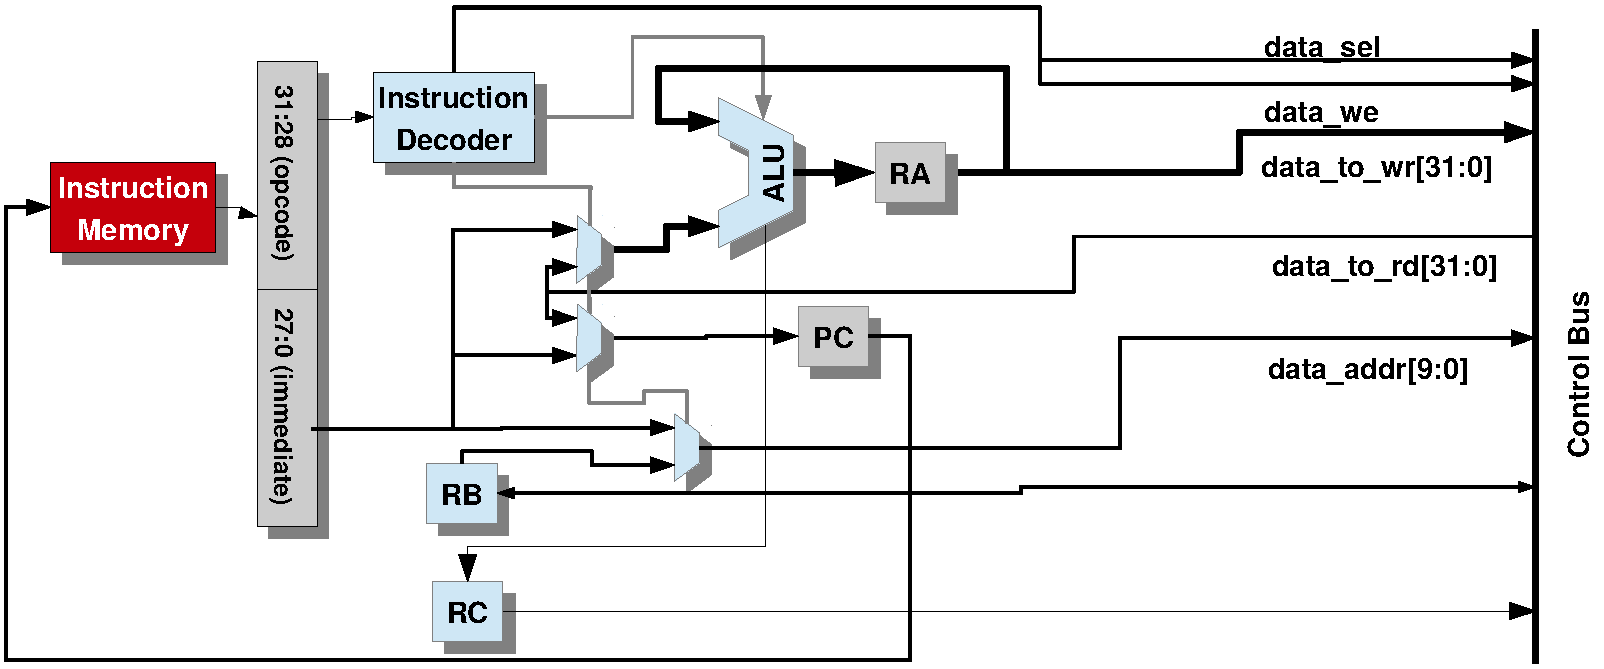
\includegraphics[width=0.9\textwidth]{Figures/bd.pdf}}
		\vspace{0cm}\caption{picoVersat Block Diagram: with registers
		(RA, RB, RC and PC), their interconnections and memory access.}
    \label{fig:bd}
\end{figure}

{\it picoVersat} is composed of four main registers:
\begin{itemize}
\item Register {\bf RA} is the accumulator and is the most relevant of the registers
in the architecture.  It can be loaded with a value read from the data interface
or with an immediate value from an instruction.  It gets the value from the
result of the operations, and is used as an operand itself along with an
immediate value or an addressed value. The value of {\bf RA} is sent to the data
interface.
%
\item Register {\bf RB}, the data pointer, is used to implement indirect loads/stores
to/from the accumulator.  This register is mapped in memory which means it is
accessed by reading/writing as if accessing the data interface.
%
\item Register {\bf RC} is the flag register, storing three operation flags which are
the negative, overflow, and carry flags.  Much like register {\bf RB}, this
register is also memory mapped but this one is mapped to a {\it read only}
section, being only set by the {\sc ALU}.  The structure used for this register
is depicted in Table~\ref{tab:flags}.  As it is shown in Table~\ref{tab:flags} some bits
are not used and could be used to implement other flags but, as of right now,
there has not been a need to add any more.

\begin{table}[!htbp]
  \centering
    \begin{tabular}{|c|c|p{7cm}|}
    \hline
    {\bf Bits} & {\bf Name} & {\bf Description} \\
    \hline \hline
     31-3 & NA & Reserved for future use\\
    \hline
     2 & Negative & Asserted if last {\sc ALU} operation generated a negative result\\
    \hline
     1 & Overflow &  Asserted if last {\sc ALU} operation generated an arithmetic overflow\\
    \hline
     0 & Carry & Asserted if last {\sc ALU} operation generated a carry\\
    \hline

    \end{tabular}
  \caption{Register C: flags}
  \label{tab:flags}
\end{table}

\item The Program Counter, {\bf PC} register, contains the next instruction to be
fetched from the Program Memory so that it can be executed.  This register
increments for every instruction, in order to fetch the next instruction except
for branch, in which the {\bf PC} register is loaded either with an immediate
present in the branch instruction, or with the value present in {\bf RB}.  These
two types of branches implement direct and indirect branches, respectively.
\end{itemize}

For increasing the frequency, by reducing the critical path, the controller
takes two clock cycles to fetch one instruction, in pipeline.  It executes every
instruction that is fetched.  In other words, it has 2 delay slots in the case
of a branch instruction.  These delay slots can be filled with a no-operation
instruction ({\sc NOP}), but the compiler/programmer can also use them to
execute useful instructions.  For instance, in the case of a {\tt for}
loop, the delay slots can be used to write the iteration count to some
register~\cite{Lopes2017}.

\subsubsection{Instruction Set}

The instruction set that is used to run {\it picoVersat} is minimalist and
has only one type.  This type has 32 bits and is divided between an
{\it opcode} and an immediate constant, like it is shown in Table~\ref{tab:if}.

\begin{table}[!htbp]
  \centering
    \begin{tabular}{|c|p{7cm}|}
    \hline
    {\bf Bits} & {\bf Description} \\
    \hline \hline
     31-28 & Operation code (opcode)\\
    \hline
     27-0 & Immediate constant \\
    \hline

    \end{tabular}
  \caption{Instruction format.}
  \label{tab:if}
\end{table}

The operations that the controller can perform are listed in
Table~\ref{tab:isa}.  The notation used for the logic, that represents the
operations, is written with {\bf C} language syntax in mind.
It is also notable that {\it Imm} represents an immediate constant and that
{\it M$[$Imm$]$} represents the contents in address {\it Imm} in memory.

\begin{table}[!htbp]
  \centering
    \begin{tabular}{|c|c|p{8cm}|}
    \hline
    {\bf Mnemonic} & {\bf Opcode} & {\bf Description} \\
    \hline \hline
\multicolumn{3}{|c|}{{\bf Arithmetic / Logic}}\\
\hline \hline
    addi  & 0x0 & RA = RA + Imm; PC=PC+1\\
    \hline
    add   & 0x1 & RA = RA + M[Imm]; PC=PC+1\\
    \hline
    sub   & 0x2 & RA = RA - M[Imm]; PC=PC+1\\
    \hline
    shft  & 0x3 & RA = (Imm $<$ 0) ? RA $<<$ 1: RA $>>$ 1; PC=PC+1\\
    \hline
    and   & 0x4 & RA = RA \& M[Imm]; PC=PC+1\\
    \hline
    xor   & 0x5 & RA = RA $\oplus$ M[Imm]; PC=PC+1\\
    \hline
\multicolumn{3}{|c|}{{\bf Load / Store}}\\
\hline \hline
    ldi   & 0x6 & RA = Imm; PC=PC+1\\
    \hline
    ldih  & 0x7 & RA[31:16] = Imm; PC=PC+1\\
    \hline
    rdw   & 0x8 & RA = M[Imm]; PC = PC+1\\
    \hline
    wrw   & 0x9 & M[Imm] = RA; PC = PC+1\\
    \hline
    rdwb  & 0xA & RA = M[RB+Imm]; PC = PC+1\\
    \hline
    wrwb  & 0xB & M[RB+Imm] = RA; PC = PC+1\\
    \hline
\multicolumn{3}{|c|}{{\bf Branch}}\\
\hline \hline
    beqi  & 0xC & RA == 0 ? PC = Imm: PC += 1; RA = RA-1\\
    \hline
    beq   & 0xD & RA == 0 ? PC = M[RB]: PC += 1; RA = RA-1\\
    \hline
    bneqi & 0xE & RA != 0 ? PC = Imm: PC += 1; RA = RA-1\\
    \hline
    bneq  & 0xF & RA != 0 ? PC = M[RB]: PC += 1; RA = RA-1\\
    \hline

    \end{tabular}
  \caption{Instruction set.}
  \label{tab:isa}
\end{table}

Additionally, the pseudo instruction {\tt nop} can be used
in assembly and is converted by the assembler.
It means No-OPeration or do nothing and is coded as {\tt addi 0}.
The instruction following a branch instruction is always executed due
to the instruction pipeline latency (delayed branch or slot).  Pad with
{\tt nop}s if no useful instructions can be executed.

This controller has the capability to work on its own, that is, the controller
can run the functions and operations that do not depend on the {\it Versat}
accelerator itself without it being connected, which allows the execution of
simple applications that do not have tight time constrains.

\subsection{Previous Compiler}

The previous compiler~\cite{Santiago2017} was made from scratch and
was based around object oriented programming languages like {\it JAVA}
and {\it C++}.  Although, it claims to be
a {\bf C++} dialect, it provides no classes, not even {\bf C} structures,
variables or declarations, and no object-oriented capabilities like
encapsulation or polymorphism.  The use of a `dot' to access object functions
({\em obj.func()}) of predefined objects extends the use of {\bf C} alike
structure addressing to a small set of compiler static dependent objects.

The compiler was developed around the idea that each component of {\it Versat}
is viewed as an object. Each function that each object can perform is called by
referencing the function within the object.  The programming is performed by
calling operations on those predefined objects.  This was a good idea but, since
a true object oriented approach is far too complex for the architecture of a
{\sc CGRA}, the result ended up looking like an object based language but not
working like one.  Instead of using a classic approach where an abstract syntax tree ({\sc AST}) is
built from syntactic description, the compiler only uses components to represent
the {\bf Versat} hardware components.


Before developing the previous compiler existing common compilers were
investigated, like {\bf gcc} or {\bf llvm}, but it was ``concluded that
these compilers are good at producing sequences of instructions but not
sequences of hardware datapaths''~\cite[p.~21]{Lopes2017}.

% these do João lopes, p.21

%Another problem this compiler has is the fact that it does not allow for the coding of some functionalities that the CGRA itself has, as well as not have an implemented optimization step in the {\it back-end} of the compilation process.
% 40KB 10.8Kl 300KB asm, with -S
Another drawback is that this compiler does not allow for the coding of some
functionalities that the {\sc CGRA} itself has, and do not have an implemented
optimization step in the {\it back-end} of the compilation process.
% 40KB 10.8Kl 300KB asm, with -S


The above problems and the aims described in the Objectives section is the
reason why the previous compiler needs to be improved, as is the purpose of this
work.  In order to achieve the objectives there were two options: continue
evolving the previous compiler by adding new functionalities, or to create a new
compiler through a different method that would be more adapted to the type of
architecture.

The first option, even though it seems to be the easiest, suffers from the
problem that it took as a base an object oriented architecture but does not work
like one. To circumvent the previous approach as well as the other problems
described earlier, a research was made in order to see if the other option was
better or worst.

The main advantage of the second option of creating a compiler not from scratch
is that it allows for the user code to be written exactly in the {\bf C}
programming language.
This is a very good advantage, not only because of the extra help given to the
programmer, but also because it would allow to make the optimization simpler.
%, since C code is researched and easier to code than.
Another good point to defend this approach is that the controller itself can
work on it's own, without the {\it Versat} accelerator, being able to run any
{\bf C} code, even if much slower that with the accelerator connected.

\section{Compilers} % 7
\label{section:compilers}
%escolha do compilador mais detalhada no final (seccao seguinte)


Since using the previous compiler as a starting point is not a good option,
existing compilers should be investigated.  First, the components of a compiler
must be analyzed.  Then, taking into account the usage of compiler components by
existing compilers, a selection of widespread compilers is analyzed.  Finally, a
comparative analysis of the most common compilers is performed in order to
select candidates suitable for conversion.  The converted compiler should
generate {\em picoVersat} assembly, identify and configure the {\em Versat} {\sc
  CGRA} architecture.

Computer programming, and processor programming in particular, is a complex and
time consuming task.  Computers execute binary code, but writing binary code is
an error prone and meticulous task reserved for very small low level
programming.  Assembly provided a textual approach to computer programming,
while keeping full control over the instruction set for a particular processor.

A compiler is a tool that allows the programmer to write abstract high-level
instructions and produces assembly code for the processor~\cite{aho06,cooper03}.
The assembler tool can then be used to transform the assembly instructions into
binary instructions of the processor.  The compiler can also perform semantic
error detection and data flow analysis, thus improving the required development
cycle and the generated code quality.  A good compiler can produce optimized
code as good, or sometimes better, than the manually written assembly
equivalent.

In order to transform a high-level programming language into assembly code, the
compiler tool is composed of two major phases: an analysis phase and a synthesis
phase.  During the analysis phase the input file is read, byte by byte, and
structured into an abstract syntax tree ({\sc AST}) containing all the relevant
information for final code generation.  The synthesis phase transforms an {\sc
  AST} into machine code assembly instructions~\cite{cooper03,appel08}.  These phases
correspond to, what is called in compiler terminology, the {\it front-end} and the
{\it back-end}, respectively.

%chap 1.2, 1.3

\subsection{Analysis}

The analysis phase is decomposed into three analysis stages: lexical,
syntactical and semantic.  The stages are pipelined in such a way that the
output of a lexical analyzer is fed into a syntactic analyzer, and the output of
the syntactic analyzer is coupled with the semantic analyzer.  At the end of the
syntactic analysis, the language in the input file is converted into an {\sc
  AST}.

\subsubsection{Lexical analysis}\label{lex}

The lexical analysis processes the input file, containing the high-level
computer program, into identifiable {\em tokens}~\cite{schreiner85,lexyacc95}.
The {\em tokens} are symbols or words that play a specific role in the input
language.  For instance, in the {\bf C} programming language, braces and
semi-columns, among others, are of particular interest~\cite{cpl}.  Other {\em
  tokens} may include identifiers, operators and language reserved keywords such
as data types or flow control.  The lexical analysis also removes information
that is irrelevant for code compilation, including comments and white-spaces.

The lexical analysis can be performed using simple and efficient algorithms
based on regular expressions.  However, as it is tedious, difficult to amend and
error prone work, lexical generator can be used to automate and simplify the
lexical generator.  The lexical analyzer generator {\bf lex}~\cite{Lesk:lex} and
its successors, like {\bf flex} or {\bf jflex}, can produce very compact and
efficient lexical analyzers from a simple description based on regular
expressions and embedded {\bf C} or {\bf C++} code.

\subsubsection{Syntactic analysis}\label{yacc}

The syntactic analysis phase structures a sequence of {\em tokens} provided by
lexical analysis into a tree of tokens~\cite{schreiner85,lexyacc95}.  The
purpose of the syntactic analysis is to check the order of the {\em tokens} and
identify the language constructs that they aim to describe.  After the syntactic
analysis the structure of the program is well defined and constructs like
expressions, instructions, functions and variable declarations have been
identified.

The syntactic analysis, as the lexical analysis, can be greatly simplified using
efficient algorithms.  However, these algorithms are more complex and time
consuming than the ones used in the lexical analysis.  These algorithms are
grouped into two different groups, {\bf LL} and {\bf LR}, depending whether the
constructs are identified {\bf L}eft-to-right or {\bf R}ight-to-left (the second
letter in the acronym, since the first reveals the {\em token} arriving order
which is always {\bf L}eft-to-right).  The syntactic analysis is described by a
context-free grammar describing the constructs of the high-level language being
processed.  Depending on the specific algorithm used to parse the grammar, a
different but equivalent grammar must be found.  The {\bf LALR(1)} algorithm,
which stands for {\bf L}ook-{\bf A}head {\bf LR} with a single lookahead {\em
  token}, allows a wide range of equivalent grammars, making the discovery of a
suitable grammar for the high-level language a simple task.

As for the lexical analysis, also the syntactic analyzer can be generated using
an automated tool from a grammar description with {\bf C} or {\bf C++} code
insert using tools like {\bf yacc}~\cite{Johnson:yacc} or {\bf
  bison}~\cite{donnelly03}.  The code insert are used to build the {\bf AST}.
Frequently, each grammar rule produces a tree node in the {\sc AST}.
Tools like {\bf antlr}, a {\bf SLL(*)} (a {\bf S}trong {\bf LL} with
arbitrary lookahead {\bf (*)} parser generator), provide mechanisms to
automate the construction of the {\sc AST}~\cite{parr07}.

\subsubsection{Semantic analysis}

The semantic analysis phase is responsible for checking if the constructs,
identified by the syntactic grammar, are accepted by the high-level language
and can be performed by the computer.  It must check if a variable was already
declared or if the operation request can be performed by the variable.  The
semantic analysis results from the fact that grammar must be context-free in
order to be processed by efficient syntactic algorithms.

The semantic analyzer scans the {\bf AST} for inconsistencies and prevents code
from being generated for erroneous programs.  Since semantic check is very
dependent on the high-level language particulars, it is usually performed by the
host language ({\bf C} or {\bf C++} in most cases) after, or even during, the
syntactic analysis.
%chap 8.1.1 - 8.1.5, 8.2.1 - 8.2.6

\subsection{Synthesis}

The synthesis phase is no longer dependent on the input high-level language.
Many compilers produce the {\sc AST} from different high-level languages,
although some languages may not generate some type of nodes.  On the other hand,
many compilers produce code for different processors and computer architectures
from the same {\bf AST}~\cite{hanson95}.

The synthesis phase is comprised of several stages: instruction selection,
instruction scheduling, register allocation, optimization, and data flow
analysis.  Code synthesis is an NP-complete problem and a particular order of
stages does not necessarily produce the best code, since a good decision in one
stage can compromise the quality of subsequent stages.  Some compilers repeat
some stages or try different approaches in order to find the best among them.

%chap 13.1, 13.2, 14 (14.1) - explicar cada um

\subsubsection{Instruction selection and scheduling}\label{burg}

Most compilers begin the synthesis phase by the instruction selection.
Instruction selection aims at finding the best processor instructions for a part
of an {\sc AST}~\cite{cooper03,Fraser:burg,Proebsting:2002}.  For instance, an
{\bf arm} processor offers a free sum ({\tt add}) for each multiplication ({\tt
  mul}) and free shift for most arithmetic instructions.  When these pairs of
instructions are found in contiguous tree nodes, a single instruction can be
produced, otherwise each node produces a processor instruction.
%More complex instructions, such as {\em load-effective-address} ({\tt lea}) in {\tt Intel-x86} processors,
An instruction selector generator is a tool based on a grammar that describes
the tree pattern that matches a given processor instruction.  In fact, the
grammar describes the target processor capabilities in terms of tree patterns.
To each tree pattern can be assigned a cost, that measures the time consumed by
the instruction execution.  The selector generator chooses
the best combination of instructions that map all the {\sc AST}, that is where
total cost is minimum.  As a result, the instruction selection produces a
sequence of target processor instructions.  The arguments of the instruction,
that is its registers, are not yet assigned.
Instruction selection can be performed by dynamic programming where the {\sc AST}
is searched twice, one for determining the instruction costs and a second to generate
the best selected instructions.
Therefor, the algorithm is linear on the number of instructions (O(N)).
The instruction selection tools, known as {\sc BURG} ({\bf B}ottom {\bf U}p
{\bf R}ewrite {\bf G}rammar), like {\tt lburg}, {\tt iburg}, {\tt monoburg}
automate the code generation process.

%This step has linear complexity (O(N)) as do most of the algorithms used in compiler development.

\paragraph{{\sc C3E} versus {\sc SSA}}

When representing abstract processor instructions there are two representations:
{\em three address instructions} ({\sc C3E}) and {\em static single assignment}
({\sc SSA})~\cite{appel08,parsons92}.
In {\sc C3E} each instruction takes up to three arguments, one of
them being the destination of the operation.  These instructions arguments are
not yet registers, since register allocation was not performed, but names of
high-level variables.  More recently, since {\sc gcc-4} and in other modern
compilers, the {\sc SSA} has been adopted because it provides a better base for
optimization, allocation and scheduling.  In {\sc SSA} each argument is tagged
with a version number and, each time the variable is reassigned, the version
number is incremented.  Therefor, two registers can contain different versions
of the same variable, allowing for a better use of common sub-expressions.
For instance, in {\tt while (*s++)} both $s_0$ and $s_1$ from $s_1 = s_0 + 1$, the old value is kept in a register for the evaluation of the condition while the new value is stored in memory.

\paragraph{Basic blocks}

A basic block is a sequence of instructions that have no labels between them,
allowing transfer of control into the block, nor have jump instructions among
them.  A jump instruction always ends a basic block.  A label always breaks a
block in two basic blocks.  Within a basic block the sequence of instructions
can be changed, as long as the argument dependencies are kept.


\paragraph{Instruction scheduling}

The scheduling is performed on code basic blocks.  The scheduling rearranges the
order of the instructions taking into account the number of available functional
units in the processor and the latency of their executions.  To each instruction
is given an available functional unit, and a simulation of the execution is
performed to determine when the functional unit is again available for the next
instruction.  For instance, when a multiplication is being performed, other
operations like sums and shifts can be done in parallel as long as there is no
dependency on the arguments.  The rearrangement of the instructions produces the
minimum sum of elapsed time, including latencies.
List scheduling is a greedy heuristic approach that performs a simulation of the
execution of a basic block instructions once (O(N)), but it is quadratic on the
number of operands (O($m^2$)), although for most operations $m$ is one or
two~\cite[p.605]{cooper03}.
For instance, when an operation requires arguments that result from a $sum$ and a $multiplication$, the $multiplication$ is performed first since it has higher latency, and the $sum$ is executed while the $multiplication$ is being performed if both operations can be paralelized.

\subsubsection{Register allocation}

Register allocation aims at finding the best use of the available machine
registers.  On machines with a small number of registers, the process is simple
since there are not that many options.  Modern {\sc RISC} machines register 
allocation, with 16 or more general purpose registers,  is both complex and central
to the efficiency of the resulting code.  Register allocation algorithms are
divided in local, within basic blocks, and global, when involving more than one
basic block.

When performing local register allocation the available registers can be freely
assigned and an optimal algorithm exist, for instance when generating code for
expressions.  Global register allocation usually sets aside some of the
registers and tries to distribute their use among the basic blocks, taking into
account their dependencies (see~Optimization and data flow analysis).
When one basic block uses more
registers, another must be sacrificed, and no optimal solutions exist.  However,
if instructions are limited to {\bf if}, {\bf do}, {\bf while} and {\bf for}
without the indiscriminate use of {\bf goto}, a good solution can be obtained.

Register allocation is based on {\tt live} or {\tt dirty} registers, those that
presently contain a useful value, and {\tt dead} or {\tt clean} registers,
those that can be assigned to new uses.
However, {\tt live} registers can contain a copy of
memory value, allowing for its use without saving, or computed values that must
first be saved before the register can be used for another purpose.  It is up to
the allocation algorithm to find the best combination of registers in order to
reduce the number of memory {\tt loads} and {\tt stores}.

Register allocation algorithms include local algorithms like {\em Sethi-Ullman}
(optimal for expressions), {\em greedy}, {\em next-use} and {\em top-down} or
{\em bottom-up} approaches.  Global allocation uses {\em linear scan} for simple
{\tt just-in-time} compilers and more complex {\em graph coloring} for optimizing
compilers.

\subsubsection{Optimization and data flow analysis} \label{dataflow}

Once the code is generated it can be rearranged.  In fact, optimization begins
with instruction selection and is present in each stage of the synthesis
phase~\cite{allen01,muchnick97}.
Simple optimizations, like {\em peephole} where a sliding window analyses
sequences of adjacent instructions, can be performed after instruction
selection when two nodes produce contiguous instructions that can be
replaced by a better one.
Data flow analysis is an optimization that searches for the best
sequencing of basic blocks, reducing the number of inter-block jumps.  Complex
compilers may provide thousands of optimizations that must be tested in order to
find out if an improvement can be achieved.

\subsection{B language compiler}

The {\bf B} programming language is the predecessor of the {\bf C} programming
language and provides a very similar syntax~\cite{lang:b}.  {\bf B} uses only an
integer data type, eliminating the need for data structures.  It provides access
to single byte characters through literals and library manipulation
routines~(see Figure~\ref{fig:blc}).  All {\bf C} operators and instructions are
present but lacks the {\bf for} construct.  Missing is also the preprocessor.

\begin{figure}[!htbp]
    \centerline{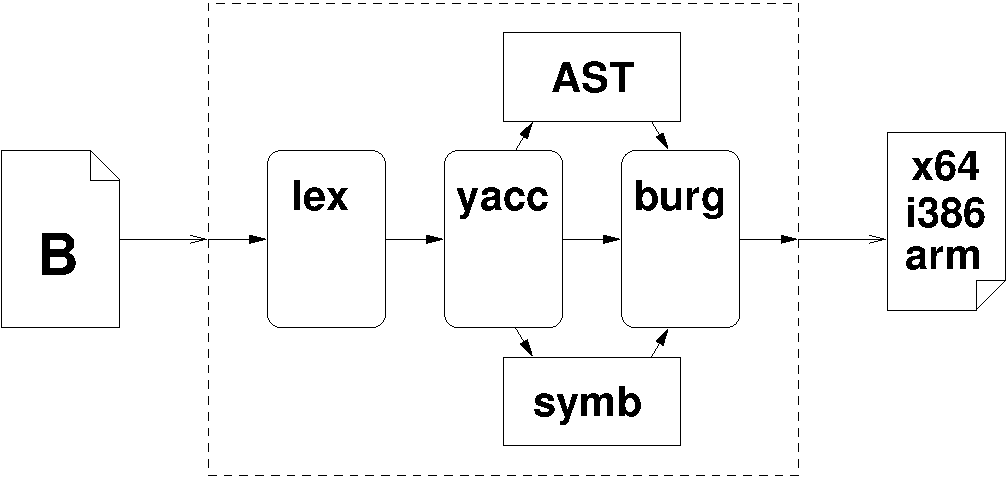
\includegraphics[height=50mm]{Figures/blc.pdf}}
    \vspace{0cm}\caption{{\bf B} language compiler.}
    \label{fig:blc}
\end{figure}

%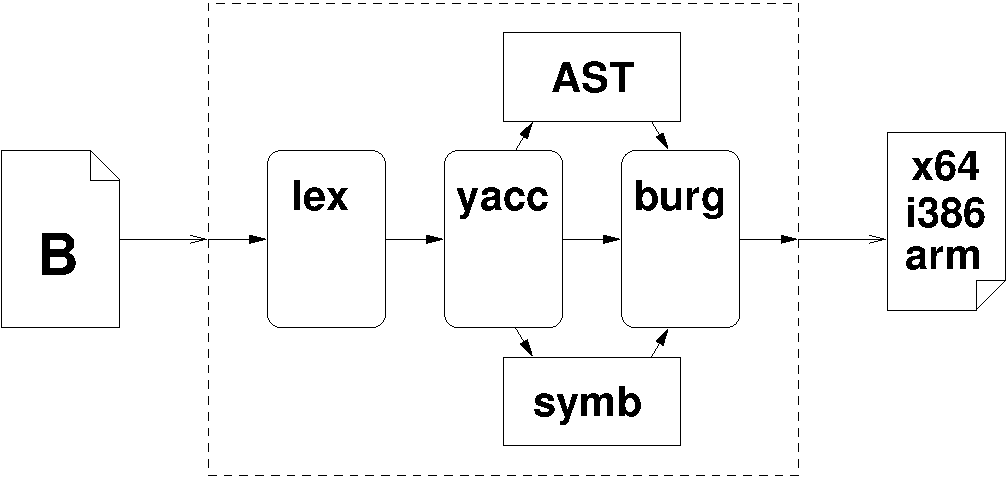
\includegraphics[height=50mm]{Figures/blc.pdf}

The  {\bf B} language compiler ({\bf blc}) is very small, under one thousand lines of
{\bf C} code with grammars for the {\bf flex}, {\bf bison} and {\bf  burg} compiler generators. %\footnote{https://github.com/pedroreissantos/B-programming-language}
New constructs can be easily added to the language, but it will no longer be {\bf B}.
There is complete access to all parts of the compiler and {\tt asm} support is provided.
%asm, with -S

\subsection{gcc}

{\bf gcc} was originally created by Richard Stallman in 1987 ({\tt 0.9 beta},
March 22) as free {\bf C} compiler~\cite{Stallman:2009}.  As of version {\tt
  1.27} (September 5, 1988) was a stable usable compiler.  In 2018 there were 4
major software releases from 3 development branches.  It includes, up to now,
494 contributors~\cite{Stallman:2018}.  The compressed ({.tar.gz}) source code
is 80MB (8.2.0), 535MB uncompressed with over 14 million lines of
code\footnote{https://gcc.gnu.org/releases.html}.  {\bf
  gcc} includes compilers for {\bf Ada}, {\bf C}, {\bf C++}, {\bf Fortran}, {\bf
  Java} and {\bf Objective C}.  It includes code generation for most 32-bit and
64-bit main stream commercial processors, including {\bf x86}, {\bf x64} and
{\bf arm}.

{\bf gcc} provides three types of intermediate languages: generic, gimple and
rtl~(see Figure~\ref{fig:Gcc}).  Generic is `language-independent way of
representing an entire function in trees', essentially a complex {\sc AST}.
Gimple is a {\bf C3E} representation, where some operations can have more than 3
arguments, in a {\bf C++} inheritance hierarchy and a 29 instruction set.  The
{\tt rtl} (Register Transfer Language) is a low-level intermediate
representation in a {\bf lisp} alike form.  Target machine descriptions can be
provided through a {\bf burg} alike file of pattern descriptions.

\begin{figure}[!htbp]
    \centerline{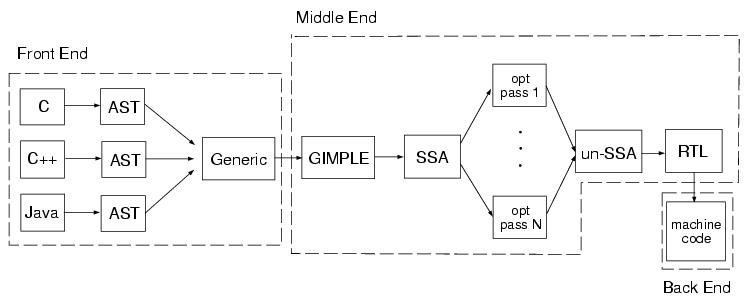
\includegraphics[height=50mm]{Figures/Gcc.jpg}}
    \vspace{0cm}\caption{{\bf Gcc} compiler.}
    \label{fig:Gcc}
\end{figure}

%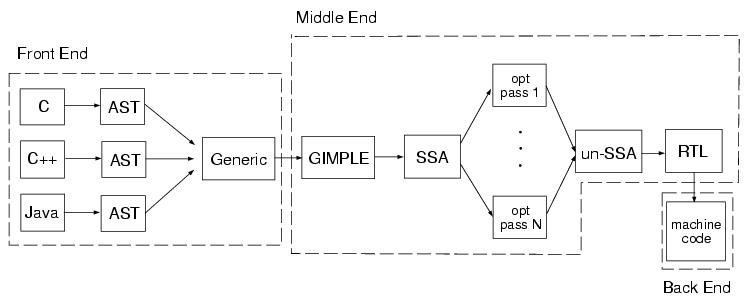
\includegraphics[height=60mm]{Figures/Gcc.jpg}

There is a book describing the compiler internals for versions 3.4 and
4.1~\cite{Stallman:2009}, although in 2018 distributions are for
versions 7, 8 and upcoming 9 (accessible in {\sc SVN})~\cite{Stallman:2018}.
The compressed ({.tar.gz}) source code is 80MB (8.2.0), 535MB.  The document for
the upcoming release 9 is essentially a listing of functions with a single line
description for each function.

%"GNU Compiler Collection Internals", Richard Stallman, Oct 2018, (9.0.0 pre-release).
%"From Source to Binary: The Inner Workings of GCC", Red Hat Magazine, number 2, Dec 2004.

The best, with thousands of generic and architecture specific optimizations,
but it is a monster!  Very big, lots of people change it and maintain
it, making the code very volatile, since the user must keep up to constant
changes in the code.  The purpose is not code optimization since {\it Versat} does
not provide alternative instructions for its operations, only {\it picoVersat}
could benefit of {\bf gcc} features.  It provides {\tt asm} support and many other
{\bf gcc} specific {\bf C} language extensions.

\subsection{llvm}

\begin{figure}[!htbp]
    \centerline{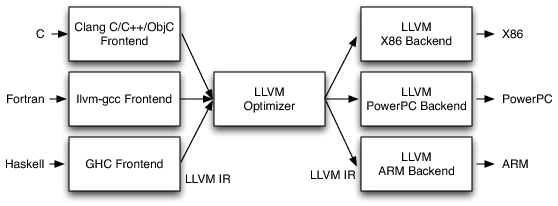
\includegraphics[height=45mm]{Figures/LLVMCompiler1.png}}
    \vspace{0cm}\caption{{\bf LLVM} compiler.}
    \label{fig:LLVM}
\end{figure}

%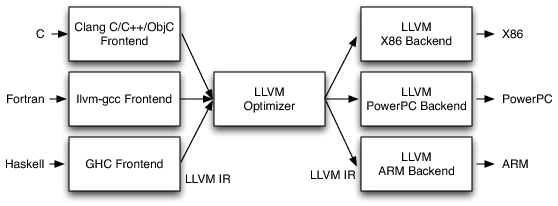
\includegraphics[height=50mm]{Figures/LLVMCompiler1.png}

{\sc LLVM} ({\em Low Level Virtual Machine}) was born as an infrastructure for
optimization from the masters thesis of Chris Lattner at the University of
Illinois at Urbana-Champaign~\cite{llvm:msc,Lattner04}.  Although an effort was
made to integrate it into {\bf gcc} it evolved into a full compiler with many
{\it front-ends}.  The first version was published Oct 24, 2003 with four releases
in 2018.  Many contributions for the compiler tool-chain were made over
the year, resulting in over 250 publications ({\tt http://llvm.org/pubs/}).

Nowadays, the code is extensive.  Only the core is 27MB compressed, resulting in
almost 7 million lines of code occupying 296 MB
(7.0.0)\footnote{http://releases.llvm.org/}.  The {\bf C} language
compiler ({\bf clang}) is roughly half the size.  Other {\it front-ends} include {\bf
  C++}, {\bf Objective C} and {\bf Fortran} among others.  It provides {\it back-ends}
for many processors: {\bf X86}, {\bf X86-64}, {\bf PowerPC}, {\bf PowerPC-64},
{\bf ARM}, {\bf Thumb}, {\bf SPARC}, {\bf Alpha}, {\bf CellSPU}, {\bf MIPS},
{\bf MSP430}, {\bf SystemZ}, and {\bf XCore}~(see Figure~\ref{fig:LLVM}).  A new
target description is provided by a declarative domain-specific language
processed by the {\bf tblgen} tool, similar to {\bf burg} grammar descriptions.
It features a stable internal instruction set implementation and documentation.

The compiler supports {\tt asm} directive extension and checks the correctness
of the embedded assembler itself.

It is still very large and difficult to manipulate.  The interface is complex,
written in {\bf C++}, but stable.  Requires a big effort for a single person for
a few months.

%"LLVM: A Compilation Framework for Lifelong Program Analysis \& Transformation"
%Chris Lattner and Vikram Adve
%Proc. of the 2004 International Symposium on Code Generation and Optimization (CGO'04), Palo Alto, California, Mar. 2004.
%
%"LLVM: An Infrastructure for Multi-Stage Optimization"
%Chris Lattner
%Masters Thesis, Computer Science Dept., University of Illinois at Urbana-Champaign, Dec. 2002.
%asm, -S, checks asm string!

\subsection{lcc}\label{lcc}

The {\bf lcc} is a {\bf C} compiler developed after the publication of the
{\bf BURG} papers by Proebstring, Hanson and Fraser in 1992, as a
demonstration of the concept~\cite{Fraser:burg,Fraser:gen92,Proebsting:2002}.
Up to that time {\it back-end}
compiler writing was an art.  The {\bf burg} concept allowed to describe the
target architectures in a single file as well as maintaining all of them in a
single executable, a retargetable compiler.  The target architecture is
selectable by a command line option.

Only the {\bf C} {\it front-end} is supported with a custom made lexical analyzer and
a {\bf yacc} parser~(see Figure~\ref{fig:lcc}).  The language is described in an
{\sc AST} with a well documented 32 instruction set.  Optimizations are
performed in the {\sc AST}, and through common sub-expression analysis, the tree
is converted into a {\bf DAG} ({\em Directed-Acyclic Graph}), although the
original tree is still accessible.

\begin{figure}[!htbp]
    \centerline{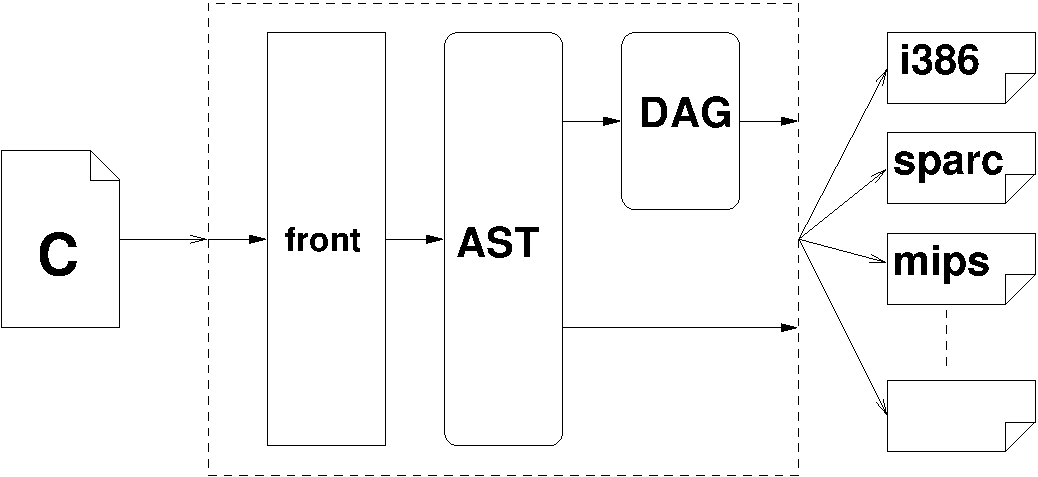
\includegraphics[height=45mm]{Figures/lcc.pdf}}
    \vspace{0cm}\caption{{\bf lcc} compiler.}
    \label{fig:lcc}
\end{figure}
%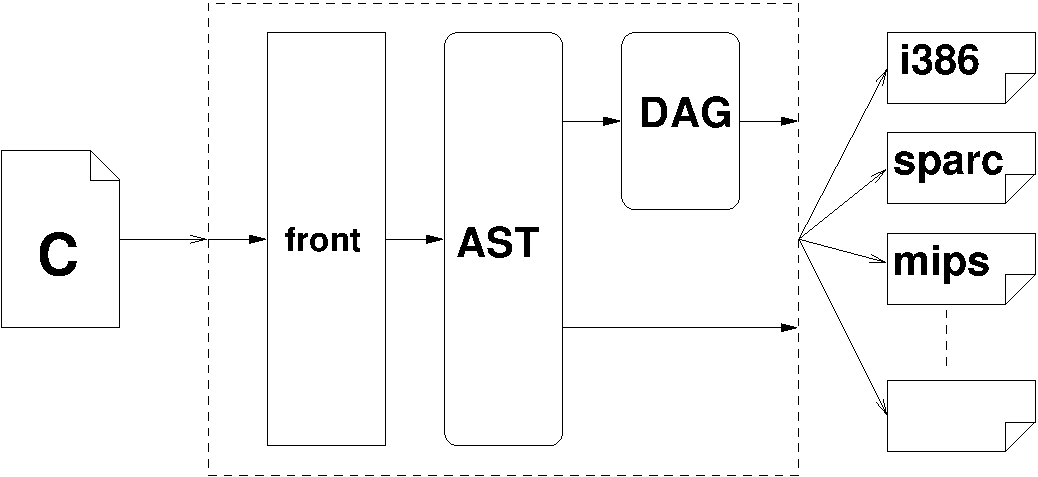
\includegraphics[height=50mm]{Figures/lcc.pdf}

A single {\bf C} {\it front-end} reduces the complexity and line count.  Simple to
introduce new {\it back-end} since it was designed to be retargetable.  A detailed and
extensive book and well defined {\it back-end} interface provide a good work
basis~\cite{hanson95}.  It provides no {\tt asm} directive and it's introduction
will require changes to core of the {\it front-end} code.  However, the compiler core
is composed of 260K lines of code and any changes should be
accessible~\footnote{https://github.com/drh/lcc}.
%626KB 260Kl 4MB
%no asm (doable)), with -S

\subsection{tcc}

The {\bf tcc} ({\em Tiny C Compiler}) is a small and fast {\bf C} compiler
written by Fabrice Bellard that began as the winner of a 2001 contest to
provide the smallest self-compiling language
({\sc OTCC})\footnote{https://bellard.org/otcc/}.
% https://bellard.org/tcc/tcc-doc.html
Now it is a full {\sc ANSI} {\bf C} compiler~\cite{Wheeler:2005} in 620KB of compressed code, totaling 105 thousand lines of code
(1.7MB)~\footnote{https://bellard.org/tcc/}.  It also claims to be 9 times faster than {\bf gcc}.  It only supports
the {\sc ANSI} {\bf C} {\it front-end} with {\it back-ends} for {\bf x86}, {\bf x64} and
{\bf arm} architectures.  The {\bf tcc} {\tt -run} option allows the code to be
compiled directly into memory, and executed without producing output files since
it includes an assembler and linker ({\em self-relying}).


On the other hand, the compiler provides few optimizations and only simple
register allocation, but the output is quite efficient for most non production
applications.  Documentation is limited but the code is manageable, however no
{\tt asm} support is provided.  Also, the compiler produces binary code
directly, not output assembler code, and it might not be easy to add assembler
support altogether.

%no asm, no -S

\subsection{Portable C Compiler}

The {\bf pcc} was developed in the 1970s by Stephen Johnson of the Bell
Labs~\cite{Johnson:1978}.
It was one of the first compilers that could target different architectures.
{\bf pcc} was the {\sc BSD Unix} {\bf C} compiler until it was replaced by
{\bf gcc}.  A 2007 rewriting ported it to {\sc C99} standard.
In the present form, {\bf pcc} was released in 2011 and supports {\bf x86}
and {\bf x64} architectures. % http://pcc.ludd.ltu.se/
It provides {\tt asm} support, but relies on rather old technology with no
instruction selection tool, such as {\bf burg}.
On the other hand it comprises only 160K lines of
code~\footnote{http://pcc.ludd.ltu.se/}.
%asm, -S
%1M, 160Kl 4MB

\subsection{Amsterdam Compiler Kit} % http://tack.sourceforge.net/ https://github.com/davidgiven/ack

The Amsterdam Compiler Kit ({\sc ACK})~\cite{Tanenbaum:1983}, developed in
early 1980s, was one of the first retargetable compilers with {\it front-ends}
for {\bf C}, {\bf Pascal}, {\bf Modula-2}, {\bf Occam}, and {\bf BASIC} as well
as {\it back-ends} for many processors and micro-processors.
The technology used is outdated but simple and no {\tt asm}
is provided~\footnote{http://tack.sourceforge.net/}.
%no asm, no -S
%4MB, 700Kl, 22MB

%Tanenbaum, Andrew S; van Staveren, H.; Keizer, E.G.; Stevenson, J.W. (1983). "A Practical Tool Kit For Making Portable Compilers". Communications of the ACM. 26 (9): 654–660. doi:10.1145/358172.358182.

\subsection{Small device C compiler} % http://sdcc.sourceforge.net/

The {\bf sdcc} is an {\sc ANSI} {\bf C} retargetable
compiler~\cite{sandeep:2000}, written by Sandeep Dutta.
It targets many microprocessors but no major processors, although it can
be retargeted for other microprocessors. The list of targets is the following.

Intel {\sc MCS51} based microprocessors (8031, 8032, 8051, 8052, etc.), Maxim
(formerly Dallas)\linebreak
{\sc DS80C390} variants, Freescale (formerly Motorola) {\sc
  HC08} based (hc08, s08), Zilog Z80 based {\sc MCUs} (z80, z180, gbz80, Rabbit
2000/3000, Rabbit 3000A, {\sc TLCS-90}), and {\sc STMicroelectronics} {\sc
  STM8}. Work on the Microchip {\sc PIC16} and {\sc PIC18} is under development.

It does not support {\tt asm} directives and the code, although large (7M lines
of code), is essentially dedicated to each specific
processor~\footnote{http://sdcc.sourceforge.net/}.
%Sep 27th, 2018: SDCC 3.8.0 released.
%no asm, with -S
%18MB compressed, 7 Mlines, 220MB

\section{{\sc CGRA} Compilers}

Unlike the previous general purpose {\bf C} language compilers, {\sc CGRA}
compilers directly address the problem of configuration and reconfiguration of a
{\sc CGRA} platform.
%ver compiladores que estao no mail (TRIPS, IMAGINE, REMARC, RICA, PADDI, Chimaera, Montium, GARP, PipeRench, EGRA, SmartCell, PADDI, Pleiades, DRRA, Redefine, Colt, Matrix, FPCA, CGRA Express, and HARTMP)
%"Coarse Grained Reconfigurable Architectures in the Past 25 Years: Overview and Classification"
%%%

% refs/2013HSPSdesutter.pdf : Coarse-GrainedReconfigurableArray Architectures
%In general, the performance obtained on a programmable processor for a certain application can be defined as the reciprocal of the application execution time.
Some {\sc CGRAs}, like {\sc ADRES}, Silicon Hive, and MorphoSys are fully
dynamically reconfigurable: exactly one full reconfiguration takes place for
every execution cycle~\cite{DeSutter2010}.  Other {\sc CGRAs} like the
KressArray are fully statically reconfigurable, meaning that the {\sc CGRA} is
configured before a loop is entered, and no reconfiguration takes place during
the loop at all~\cite{DeSutter2010}.  Still other architectures feature a hybrid
reconfigurability. The RaPiD architecture features partial dynamic
reconfigurability, in which part of the bits are statically reconfigurable and
another part is dynamically reconfigurable and controlled by a small
sequencer~\cite{DeSutter2010}.  Most compiler research has been done to generate
static schedules for {\sc CGRAs}~\cite{DeSutter2010}.  Not enough details are
available in the descriptions of the compiling techniques, and few techniques
have been tried on a wide range of {\sc CGRA} architectures~\cite{DeSutter2010}.
For that reason, it is very difficult to compare the efficiency, effectiveness
and user interface of the different techniques, this is, compilation time,
quality of the generated code, and how easy it is to use and to port code to the
language used, respectively~\cite{Tuhin08}.

There are frameworks that try to compile code in usual languages to {\sc CGRAs}.
Most of these frameworks have however some limitations that do not allow them to
adapt the code fully to {\sc CGRAs}' purposes.  For example, the {\sc IMPACT}
compiler framework is used in order to parse {\bf C} source code and get the
Intermediate Representation ({\sc IR})~\cite{Mei03}.  We can then change what
the {\it back-end} does to this {\sc IR}, to get the desired result.  However,
because of the {\sc IMPACT} {\it front-end}, most algorithms can only handle
inner loops of loop nests~\cite{Mei03}.  And since changing the {\it front-end}
as well as the {\it back-end} is the same as creating a new compiler, most of
these frameworks have problems when there is a need to really adapt the code not
made in the specific assembly language of the {\sc CGRA} supposed to run the
code.

% refs/04b_2.pdf : Exploiting Loop-Level Parallelism on Coarse-Gained Reconfigurable Architectures Using Modulo Scheduling
%Arquitectures often consist of tens to hundreds of FUs that are capable of executiong word, or even subword level operations instead of bit-level ones, which are usually found in FPGAs.

%Some use structure (GUI based) design tools to manually generate design (limits size of desing)[19, 5].
%Some use Instruction Level Paralelism (ILP) (limited scope and doesn't use architecture efficiently which means it can not reach a higher level of paralelism than a VLIW)[4, 12].
%Some use Loop-Level Paralelism (LLP), applying pipelining (suffers from applicability limitations)[3, 9, 18].

%Limitations:
%It's more time consuming compared to a typical scheduling algorithm of a compiler.
%Can not handle pipelined FUs and limited register files.
%Overall negative impact on the performance of the application.


% refs/99.pdf : Graph Minor Approach for Application Mapping on CGRAs

Nowadays most of the algorithms used for {\sc CGRAs} are adaptations of the ones
used for {\sc FPGAs} but, since the structure is not the same, this approach is
not the most efficient and/or effective~\cite{Chen14}.

%The most widely applicable static scheduling techniques use different forms of Modulo Resource Routing Graphs (MRRGs).

\subsection{Comparative Analysis}

Compilers are complex tools.  However, if the target processor is simple and the
high-level language is limited, a simple compiler can be developed in a few
months, using the right tools.  For large and complex languages like {\bf C},
with a large population of skilled programmers, a number of freely available
compilers exist.  The development of a compiler, even with powerful tools, is a
very complex and time consuming task, that usually involves tens of persons.
For large and complex languages like {\bf C} the use of an existing
infrastructure is of prime importance.

The {\bf B} programming language is a good choice if changes to the {\it front-end} of
the compiler are necessary, since changing the {\it front-end} as well as the {\it back-end}
is essentially writing a completely new compiler.

More complex languages, like {\bf C++}, are an overkill for a processor with
limited memory like {\it Versat} since with its memory limitations it will not
be able to run large object-oriented programs.

% why was lcc the choice... (in next section)
